\documentclass[tikz,border=1.8mm]{standalone}

\definecolor{fvmadaptedge}{HTML}{8A7E7E}
\definecolor{externalface}{HTML}{8FB9E8}
\definecolor{nodefill}{HTML}{FFFFFF}
\usetikzlibrary{arrows.meta,calc}

\begin{document}
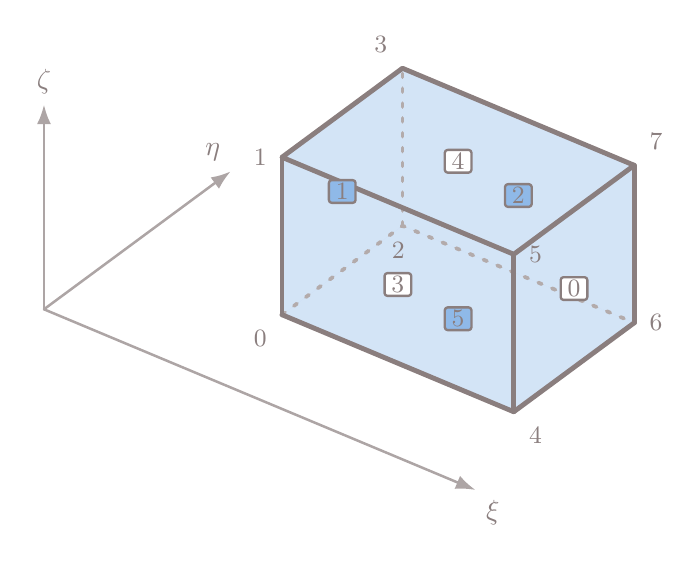
\begin{tikzpicture}[
  x={(20.3mm,-8.5mm)},
  y={(15.3mm,11.3mm)},
  z={(0mm,20mm)},
  line join=round,
  line cap=round,
  outer/.style={draw=fvmadaptedge,line width=0.62mm},
  hidden/.style={draw=fvmadaptedge!65,line width=0.48mm,loosely dotted},
  face/.style={fill=externalface,fill opacity=0.22,draw=none},
  axis/.style={draw=fvmadaptedge!70,line width=0.32mm,-{Latex[length=2.5mm,width=1.8mm]}},
  nodelabel/.style={font=\small,text=fvmadaptedge},
  facelabel/.style={rectangle,rounded corners=1.0pt,draw=fvmadaptedge,line width=0.30mm,fill=nodefill,inner xsep=2.5pt,inner ysep=1.2pt,font=\small,text=fvmadaptedge},
  occludedfacelabel/.style={rectangle,rounded corners=1.0pt,draw=fvmadaptedge,line width=0.30mm,fill=externalface,inner xsep=2.5pt,inner ysep=1.2pt,font=\small,text=fvmadaptedge},
  axislabel/.style={font=\normalsize,text=fvmadaptedge}
]
  % HexCell local node coordinates:
  % node = 4*xi + 2*eta + zeta.
  \coordinate (N0) at (0,0,0);
  \coordinate (N1) at (0,0,1);
  \coordinate (N2) at (0,1,0);
  \coordinate (N3) at (0,1,1);
  \coordinate (N4) at (1.45,0,0);
  \coordinate (N5) at (1.45,0,1);
  \coordinate (N6) at (1.45,1,0);
  \coordinate (N7) at (1.45,1,1);

  \coordinate (Oaxis) at (-1.15,-0.45,-0.20);
  \draw[axis] (Oaxis) -- (1.55,-0.45,-0.20)
    node[axislabel,below right] {$\xi$};
  \draw[axis] (Oaxis) -- (-1.15,1.10,-0.20)
    node[axislabel,above left] {$\eta$};
  \draw[axis] (Oaxis) -- (-1.15,-0.45,1.10)
    node[axislabel,above] {$\zeta$};

  \path[face] (N0) -- (N4) -- (N6) -- (N2) -- cycle;
  \path[face] (N1) -- (N5) -- (N7) -- (N3) -- cycle;
  \path[face] (N0) -- (N4) -- (N5) -- (N1) -- cycle;
  \path[face] (N4) -- (N6) -- (N7) -- (N5) -- cycle;
  \path[face] (N6) -- (N2) -- (N3) -- (N7) -- cycle;
  \path[face] (N2) -- (N0) -- (N1) -- (N3) -- cycle;

  \draw[hidden] (N0) -- (N2) -- (N6);
  \draw[hidden] (N2) -- (N3);

  \draw[outer] (N0) -- (N4) -- (N6);
  \draw[outer] (N1) -- (N5) -- (N7) -- (N3) -- cycle;
  \draw[outer] (N0) -- (N1);
  \draw[outer] (N4) -- (N5);
  \draw[outer] (N6) -- (N7);

  \node[nodelabel,below left=2pt] at (N0) {0};
  \node[nodelabel,left=2pt] at (N1) {1};
  \node[nodelabel,below left=2pt] at ($(N2)+(0.08,0.04,0)$) {2};
  \node[nodelabel,above left=2pt] at (N3) {3};
  \node[nodelabel,below right=2pt] at (N4) {4};
  \node[nodelabel,right=2pt] at (N5) {5};
  \node[nodelabel,right=2pt] at (N6) {6};
  \node[nodelabel,above right=2pt] at (N7) {7};

  \node[facelabel] at (1.45,0.50,0.50) {0};
  \node[occludedfacelabel] at (0.00,0.50,0.50) {1};
  \node[occludedfacelabel] at (0.725,1.00,0.50) {2};
  \node[facelabel] at (0.725,0.00,0.50) {3};
  \node[facelabel] at (0.725,0.50,1.00) {4};
  \node[occludedfacelabel] at (0.725,0.50,0.00) {5};
\end{tikzpicture}
\end{document}
